\documentclass[11pt,fleqn]{article}
\usepackage[margin=1in]{geometry}
\usepackage{tikz}
\usepackage{mathtools}
\usepackage{longtable}
\usepackage{enumitem}
\usepackage{hyperref}
%\usepackage[dvips]{graphics}
%\usepackage[table]{xcolor}
%\usepackage{amssymb}
\usepackage{float}
%\usepackage{subfig}
\usepackage{booktabs}
\usepackage{subcaption}

\usepackage[normalem]{ulem}

\usepackage{multicol}
\usepackage{txfonts}
\usepackage{amsfonts}
%\usepackage{natbib}
\usepackage{apacite}
\usepackage{gb4e}
\usepackage[all]{xy}
\usepackage{rotating}
\usepackage{tipa}
\usepackage{multirow}
\usepackage{authblk}
\usepackage{url}
\usepackage{pdflscape}
\usepackage{rotating}
\usepackage{adjustbox}
\usepackage{array}

\definecolor{Pink}{RGB}{255,50,170}
\newcommand{\jd}[1]{\textcolor{Pink}{[jd: #1]}}  

\newcommand{\jt}[1]{\textbf{\color{blue}JT: #1}}

\newcommand{\tableref}[1]{Tab.~\ref{#1}}
\newcommand{\figref}[1]{Fig.~\ref{#1}}

\def\bad{{\leavevmode\llap{*}}}
\def\marginal{{\leavevmode\llap{?}}}
\def\verymarginal{{\leavevmode\llap{??}}}
\def\swmarginal{{\leavevmode\llap{4}}}
\def\infelic{{\leavevmode\llap{\#}}}

\definecolor{airforceblue}{rgb}{0.36, 0.54, 0.66}
%\definecolor{gray}{rgb}{0.36, 0.54, 0.66}

\newcommand{\dashrule}[1][black]{%
  \color{#1}\rule[\dimexpr.5ex-.2pt]{4pt}{.4pt}\xleaders\hbox{\rule{4pt}{0pt}\rule[\dimexpr.5ex-.2pt]{4pt}{.4pt}}\hfill\kern0pt%
}

\setlength{\parindent}{.3in}
\setlength{\parskip}{0ex}

\newcommand{\yi}{\'{\symbol{16}}}
\newcommand{\nasi}{\~{\symbol{16}}}
\newcommand{\hina}{h\nasi na}
\newcommand{\ina}{\nasi na}

\newcommand{\foc}{$_{\mbox{\small F}}$}

\hyphenation{par-ti-ci-pa-tion}

%\setlength{\bibhang}{0.5in}
%\setlength{\bibsep}{0mm}
%\bibpunct[:]{(}{)}{,}{a}{}{,}

\newcommand{\6}{\mbox{$[\hspace*{-.6mm}[$}} 
\newcommand{\9}{\mbox{$]\hspace*{-.6mm}]$}}
\newcommand{\sem}[2]{\6#1\9$^{#2}$}
\renewcommand{\ni}{\~{\i}}

\newcommand{\citepos}[1]{\citeauthor{#1}'s \citeyear{#1}}
\newcommand{\citeposs}[1]{\citeauthor{#1}'s}
\newcommand{\citetpos}[1]{\citeauthor{#1}'s \citeyear{#1}}

\newcolumntype{R}[2]{%
    >{\adjustbox{angle=#1,lap=\width-(#2)}\bgroup}%
    l%
    <{\egroup}%
}
\newcommand*\rot{\multicolumn{1}{R{90}{0em}}}% no optional argument here, please!

\title{Prior probability predicts projection}
%\title{Higher-probability content is more projective than lower-probability content}

%\thanks{For helpful comments on the research presented here, we thank the audience at the 2018 Annual Meeting of XPRAG.de and at the University of T\"ubingen. We gratefully acknowledge financial support for this research from {\em National Science Foundation} grant BCS-1452674 (JT) and the Targeted Investment for Excellence Initiative at The Ohio State University (JT). IGOR Tuebingen}}

\author{Author(s)}

%\author[$\bullet$]{Judith Degen}
%\author[$\circ$]{Judith Tonhauser}

%\affil[$\bullet$]{Stanford University}
%\affil[$\circ$]{The Ohio State University / University of Stuttgart}

\renewcommand\Authands{ and }

\begin{document}

%\tableofcontents
%\newpage

\maketitle

\begin{abstract}

Beliefs about the world affect language processing and utterance interpretation in a variety of empirical domains. In three experiments, we tested whether subjective beliefs about the probability of world states influence \emph{projection}, that is, listeners' inferences about speaker commitment to those world states. We find that prior beliefs predict projection both at the group and at the by-participant level: the higher the prior belief in a world state, the more speakers are taken to be committed to it. This result highlights the importance of combining formal analyses of projection with cognitive theories of language understanding.  \jt{(4,098 words)}

\end{abstract}

% Brief research report: up to 4,000 words
% word count includes abstract, main body and figure captions, but not references or supplement

\section{Introduction}

Psycholinguistic work has documented a wide variety of ways in which probabilistic beliefs about the world, often termed ``world knowledge", affect  language processing  \cite<e.g.,>{chambers-etal02,hagoort-etal2004,hald-etal2007,warren2007}, including syntactic ambiguity resolution \cite<e.g.,>{chambers-etal04,bicknell-rohde2009}, reference resolution \cite<e.g.,>{winograd1972, hanna-tanenhaus04}, genericity \cite<e.g.,>{tessler-goodman2019},  scalar implicature \cite<e.g.,>{degen-etal2015}, underinformativity implicatures \cite{kravtchenko2015}, and the production of redundant referring expressions \cite{mitchell2013, westerbeek2015, Rubio2016, DegenEtAl2020}. In contrast, formal linguistic research on meaning in the tradition of \citeA{montague73}, which is devoted to specifying how meanings of expressions are computed from the meanings of the parts of the expressions, the way the parts are combined, and the contexts in which the expressions are used, has traditionally sidelined the importance of world knowledge\jt{need to check Dowty 1979, Thomason 1974 introduction to Montague collection, Word meaning entry in SEP; Hobbs World knowledge and word meaning}\footnote{Because ``knowledge" implies justified true belief but subjective beliefs need not be accurate to affect language processing in systematic ways, we henceforth avoid the term ``world knowledge" and instead refer to ``(subjective prior) beliefs about the world."}   In this paper, we provide empirical evidence from American English that \emph{projection}, a key topic in linguistic research on meaning, is systematically affected by listeners'\footnote{We include readers, writers, and signers in the terms ``listener" and ``speaker."} subjective beliefs about the world, suggesting that the computation of meaning must take into account beliefs about the world. We provide a sketch of such an account at the end of this paper. \jd{make sure you do -- link up to prior in RSA} 

To introduce projection, consider first that listeners regularly draw inferences about whether speakers are committed to utterance content. For instance, two contents that a speaker who utters \emph{Sam knows that it's raining} is typically taken to be committed to are the following: (i) the content of the complement of {\em know}, that it's raining, and (ii) the content of the matrix clause, that Sam knows (i). In formal research on meaning, the inference to (i) is attributed to the speaker having asserted the sentence, and the inference to (ii) is attributed to the lexical meaning of {\em know}, specifically, that only true content can be known \cite<e.g.,>{ccmg90}. The puzzle is that the inference to (ii) persists even when the speaker inquires about what Sam knows, as in {\em Does Sam know that it's raining?}, or when the speaker denies Sam's knowledge, as in {\em Sam doesn't know that it's raining}. Because Sam's knowledge is questioned or even denied in these variants, that is, the inference to (i) does not persist, these inferences to (ii) cannot be attributed to the aforementioned lexical meaning of {\em know}. Speaker commitment to utterance content that occurs in a negated sentence or a question is called projection in formal research on meaning, which aims to explain why content projects \cite<e.g.,>{langendoen-savin71,beaver-geurts-sep}.



%Inferences about speaker commitment are illustrated in (\ref{know}). A speaker who utters (\ref{ass}) is typically taken to be committed to the truth of the content of the complement of {\em know}, that it is raining. This inference is captured by assuming that the content of the complement (henceforth, CC) of {\em know} is an entailment. In (\ref{pq}) and (\ref{neg}), {\em know} is realized in a polar question and in the scope of negation, respectively: Because the CC is not entailed here, inferences that a speaker who utters (\ref{pq}) or (\ref{neg}) is committed to the CC can therefore not be due entailment. Instead, such inferences are attributed to the projection of the CC (e.g., \citeNP{langendoen-savin71,beaver-geurts-sep}).
%
%\begin{exe}
%\ex\label{know}
%\begin{xlist}
%\ex\label{ass} Sam knows that it's raining.
%\ex\label{pq} Does Sam know that it's raining?
%\ex\label{neg} Sam doesn't know that it's raining.
%\end{xlist}
%\end{exe}






%\begin{itemize}
%
%\item Altmann \& Kamide 1999: knowledge about lexical meaning, e.g., {\em eat} takes an edible theme, {\em move} can take a broader range of themes
%
%\item Chambers et al 2002, 2004: affordances of task-related objects, e.g., whether a container is big enough for an object to be placed inside; that an egg in a bowl can be poured but an egg in its shell cannot
%
%\item Bicknell \& Rohde 2009: knowledge of typical events and typical relationships between event participants, e.g., a kid's father is more likely to be criticized for kid's behavior than kid's orthodontist
%
%\item Degen et al 2015: listeners' world knowledge, prior beliefs about how objects behave, e.g., that marbles sink when thrown into water
%
%\item Kravtchenko \& Demberg 2015: knowledge of mutually known and highly events (e.g., paying) that are part of scripts (e.g., grocery shopping)
%
%\item Tessler \& Goodman 2019: 
%
%\end{itemize}

Recent experimental work has found that projection appears to be gradient rather than an all-or-none phenomenon: listeners' inferences about speaker commitment to utterance content vary in strength and are affected by contextual factors including the discourse status of the CC and the prosody of the utterance (for an overview see \citeNP{tbd-variability}). The hypothesis that listeners' prior beliefs influence projection was initially put forth by \citeA{stevens-etal2017} and \citeA{tbd-variability}, who observed by-item projection variability for different CCs of clause-embedding predicates like \emph{know} and \emph{discover}. They argued that one source of the observed variability may be that more a priori likely content ({\em Kim flew to New York}) projects more strongly than less a priori likely content  ({\em Kim flew to the moon}) when realized as the CC of a clause-embedding predicate (as in \emph{Did John discover that Kim flew to New York/the moon?}). This idea can straightforwardly be made sense of under recent Bayesian accounts that treat pragmatic utterance interpretation as a matter of combining uncertain prior beliefs about the world with uncertain beliefs about likely speaker production choices via Bayes' rule \cite{GoodmanFrank2016, degen-etal2015}: a CC that is more likely a priori (\emph{before} observing an utterance) is also more likely a posteriori (\emph{after} observing an utterance), even if the particular predicate biases the listener away from taking the speaker to be committed to the CC.

%\citeNP{stevens-etal2017} investigated the projection of the prejacent of manner adverb sentences; for instance, the content that Masha ran of the negated sentence {\em Masha didn't run quickly}. They hypothesized that the observed by-item variability might be due to prejacents differing in their prior probability and higher prior probability contents being more projective. \citeNP{tbd-variability} investigated the projection of content associated with 19 American English expressions, including the content of the complement of clause-embedding predicates like {\em know}, illustrated in (\ref{know}), and the prejacent of {\em stop}; for instance, the content that Mary's daughter has been biting her nails of the polar question {\em Has Mary's daughter stopped biting her nails?}. These authors, too, hypothesized that prior probability influences projection (p.500), as formulated in the hypothesis in (\ref{hyp}):

%Like \citeNP{stevens-etal2017}, \citealt[500]{tbd-variability} hypothesized that ``the projectivity of content may depend on the prior probability of the event described by the expression that conveys the content, such that content conveyed by expressions that describe more a priori likely events may be more likely to project''.

%\begin{exe}
%\ex\label{stop} Has Mary's daughter stopped biting her nails?
%\begin{xlist}
%\ex Mary's daughter stopped biting her nails.
%\ex Has Mary's daughter stopped biting her nails?
%\end{xlist}
%\end{exe}

%stop nails 0.79
%Has Mary?s daughter stopped biting her nails?
%Mary's daughter has been biting her nails
%stop play 0.89
%Did Jack stop playing outside with the kids?
%Jack was playing outside with the kids


%investigated the projection of the prejacent of utterances of manner adverb sentences, illustrated in (\ref{manner}). An utterance of (\ref{manner}a) implies both the prejacent, that Masha ran, and that her running was done in a quick manner. The prejacent is projective because it may also be implied by an utterance of the negated variant of (\ref{manner}a) given in (\ref{manner}b), especially when the adverb is produced with prosodic emphasis. 
%
%\begin{exe}
%\ex\label{manner} \citealt[1144]{stevens-etal2017}
%\begin{xlist}
%\ex Masha ran quickly.
%\ex Masha didn't run QUICKLY.
%\end{xlist}
%\end{exe}
%\citeNP{stevens-etal2017} observed by-item variability in the projection of the prejacent and suggested that this variability may be due to listeners having different prior probabilities about the prejacent.

% jd commented out:
%\begin{exe}
%\ex\label{hyp} {\bf Hypothesis:} The higher the prior probability of content, the more projective the content.
%\end{exe}

There is conflicting evidence for the hypothesis that prior beliefs influence projection. Support for the hypothesis comes from \citeA{mahler2020}, who investigated the projection of politically charged CCs of 
English clause-embedding predicates. For example, the politically charged content in (\ref{mahler-stim}) is that Obama improved/damaged the American economy. The prior probability of the content was manipulated by the speaker (Cindy in (\ref{mahler-stim})) speaking at the club meeting of either the College Republicans or Democrats.

\begin{exe}
\ex\label{mahler-stim} Cindy, at the College Republicans/Democrats club meeting: \\ Ben doesn't know that\ldots
\begin{xlist}
\ex \ldots Obama improved the American economy.
\ex \ldots Obama damaged the American economy. \hfill \cite[784f.]{mahler2020}
\end{xlist}
\end{exe}
Higher prior probability content (e.g., a liberal content like (\ref{mahler-stim}a) uttered by a Democrat) was more projective than a lower prior probability content (e.g., a liberal content uttered by a Republican). 

In contrast, \citeA{lorson2018} did not find empirical support for the hypothesis that listeners' prior beliefs influence projection %in (\ref{hyp}). 
in a study of the effect of prior probability on the projection of the pre-state content of the English change of state verb {\em stop}. Prior probability was manipulated through gender stereotypes reported in \citeA{boyce-etal2018}. For instance, because men are more likely than women to be plumbers, the pre-state content of (\ref{lorson-stim}a), that James has worked as a plumber, was hypothesized to be more projective than the pre-state content of (\ref{lorson-stim}b), that Linda has worked as a plumber.

\begin{exe}
\ex\label{lorson-stim} 
\begin{xlist}
\ex Did James stop working as a plumber?
\ex Did Linda stop working as a plumber? \hfill \cite[38]{lorson2018}
\end{xlist}
\end{exe}

Several differences between \citeposs{mahler2020} and \citeposs{lorson2018} investigations could be implicated in the differential support for the hypothesis: a) the projective content investigated (contents of complements vs.\ pre-state content of {\em stop}); b) negated sentences vs.\ questions; c) the manipulation of the prior probability (political party affiliation vs.\ gender stereotypes); and d) how explicitly the prior-manipulating information was provided to participants (statement of political party affiliation vs.\  use of a male or female name to indicate gender). The three experiments reported on in this paper provide additional support for the hypothesis that prior beliefs influence projection. Our experiments included 20 clause-embedding predicates (rather than just 7, as in \citeNP{mahler2020}) and the prior belief manipulation involved 20 properties of individuals (rather than just political party affiliation, as in \citeNP{mahler2020}, or gender, as in \citeNP{lorson2018}). Furthermore, our experiments tested the hypothesis both at the level of the individual and of the group. Exp.~1 (section \ref{s2}) investigated the effect of prior beliefs on projection by measuring prior probability of contents and projection in a within-participant design. This design allowed us to investigate whether individual participants' beliefs affected their projection ratings. In Exps.~2 (section \ref{s3}), prior probability and projection were measured in separate groups, as in \citeNP{mahler2020} and \citeNP{lorson2018}. In both experiments, more a priori likely contents were more likely to project. We reflect on the implications of this result for theories of meaning and language processing in section \ref{s4}. 

\section{Experiment 1}\label{s2}

This experiment tested whether higher prior probability content is more likely to project. Prior probability and projection ratings were collected for the contents of 20 clauses that realized the complements of 20 clause-embedding predicates.\footnote{\label{f-github}The experiments, data and R code for generating the figures and analyses of the experiments reported on in this paper are available at [redacted for review]. Exp.~1 was pregistered: [link removed for review]. All experiments were conducted with approval from the IRB of [university redacted] and informed consent was obtained.\jd{i think there's a way of anonymizing osf links?}}
%\url{https://github.com/judith-tonhauser/factivity}.}  

 %
\paragraph{Participants} 300 participants with U.S.\ IP addresses and at least 99\% of previous HITs approved were recruited on Amazon's Mechanical Turk platform (ages: 18-82, median: 35.5; 119 female, 179 male, 1 other, 1 undeclared). They were paid \$1.80.

\paragraph{Materials and procedure} The prior probability and projection of the contents of 20 clauses were measured in separate blocks. Each clause (e.g., \emph{Julian dances salsa}) was paired with two facts between participants: The content of the clause was expected to have a higher prior probability in the presence of one fact (e.g., \emph{Julian is Cuban}) than of the other (e.g., \emph{Julian is German}). See Supplement \ref{a-stim} for the full set of clauses and facts. 

In the prior block, the 20 clauses were realized as the complements of {\em How likely is it that\ldots?}~questions. As shown in Fig.~\ref{fig-exp1-prior}, each target stimulus consisted of one of the two facts for that clause and the {\em How likely is it that\ldots?} question. There were a total of 40 target stimuli in the prior block. Participants were told to read facts and to assess the likelihood of events, given those facts. They gave their responses on a slider marked `impossible' at one end (coded as 0) and `definitely' at the other (coded as 1).

In the projection block, the target stimuli consisted of a fact and a polar question that was uttered by a named speaker, as shown in Fig.~\ref{fig-exp1-projection}. The polar questions were formed by realizing the 20 clauses as the complements of the 20 clause-embedding predicates in Fig.~\ref{fig-exp1-preds}.\footnote{The 20 predicates include a cross-section of English clause-embedding predicates: They include cognitive predicates (e.g., {\em know}), emotive predicates (e.g., {\em be annoyed}), communication predicates (e.g., {\em announce}), and inferential predicates (e.g., {\em prove}). In much formal research on meaning, only predicates assumed to be factive (like {\em know}) are considered with respect to projection, to the exclusion of predicates assumed to be non-factive (like {\em think}). The results of our experiments confirm \citepos{mahler2020} result that prior probability influences the projection of the content of the complement of both types of predicates. For discussion of the distinction see \citeA{tonhauser-degen-factive}.} There were a total of 800 target stimuli in the projection block. Participants were told to imagine that they are at a party and that, on walking into the kitchen, they overhear somebody ask somebody else a question. As in \citepos{mahler2020} and \citepos{lorson2018} experiments, participants were asked to rate whether the speaker was certain of the content of the complement, taking into consideration the fact that was presented. They gave their responses on a slider marked `no' at one end (coded as 0) and `yes' at the other (coded as 1), as shown in \figref{fig-exp1-projection}. 

%\begin{exe}
%\ex\label{stim} 
%\begin{xlist}
%\ex {\bf Fact (which Carol knows):} Julian is Cuban.  \\ 
%{\bf Carol:} Does Sandra know that Julian dances salsa?
%\ex {\bf Fact (which Carol knows):} Julian is German.  \\ 
%{\bf Carol:} Does Sandra know that Julian dances salsa?
%\end{xlist}
%\end{exe}


%\begin{exe}
%\ex\label{target}  
%\begin{xlist}
%\ex {\bf Fact:} Julian is Cuban. \\ How likely is it that Julian dances salsa?
%\ex {\bf Fact:} Julian is German.  \\ How likely is it that Julian dances salsa?
%\end{xlist}
%\end{exe}

The projection block also included 6 control trials, which functioned as attention checks. The content of these items was expected not to project: For example, in Fig.~\ref{fig-exp1-projection-control}, the speaker is not committed to the main clause content, that Zack is coming to the meeting tomorrow. The same 6 main clauses were also used to form 6 filler trials in the prior block; a sample item is given in Fig.~\ref{fig-exp1-prior-filler}. These filler items were not used to assess participants' attention. For the full set of items see Supplement \ref{a-stim}.


Each participant's stimulus set was semi-randomly generated by first randomly pairing up the 20 predicates and clauses. Half of the items were then randomly assigned the respective clause's higher-probability fact, and half its lower-probability fact. Participants completed a total of 52 trials: 20 target trials in each block, 6 control trials in the projection block, and 6 filler trials in the prior block. Block order and within-block trial order were randomized.

\begin{figure}[h!]
\centering

\begin{subfigure}[t]{0.5\textwidth}
        \centering
\fbox{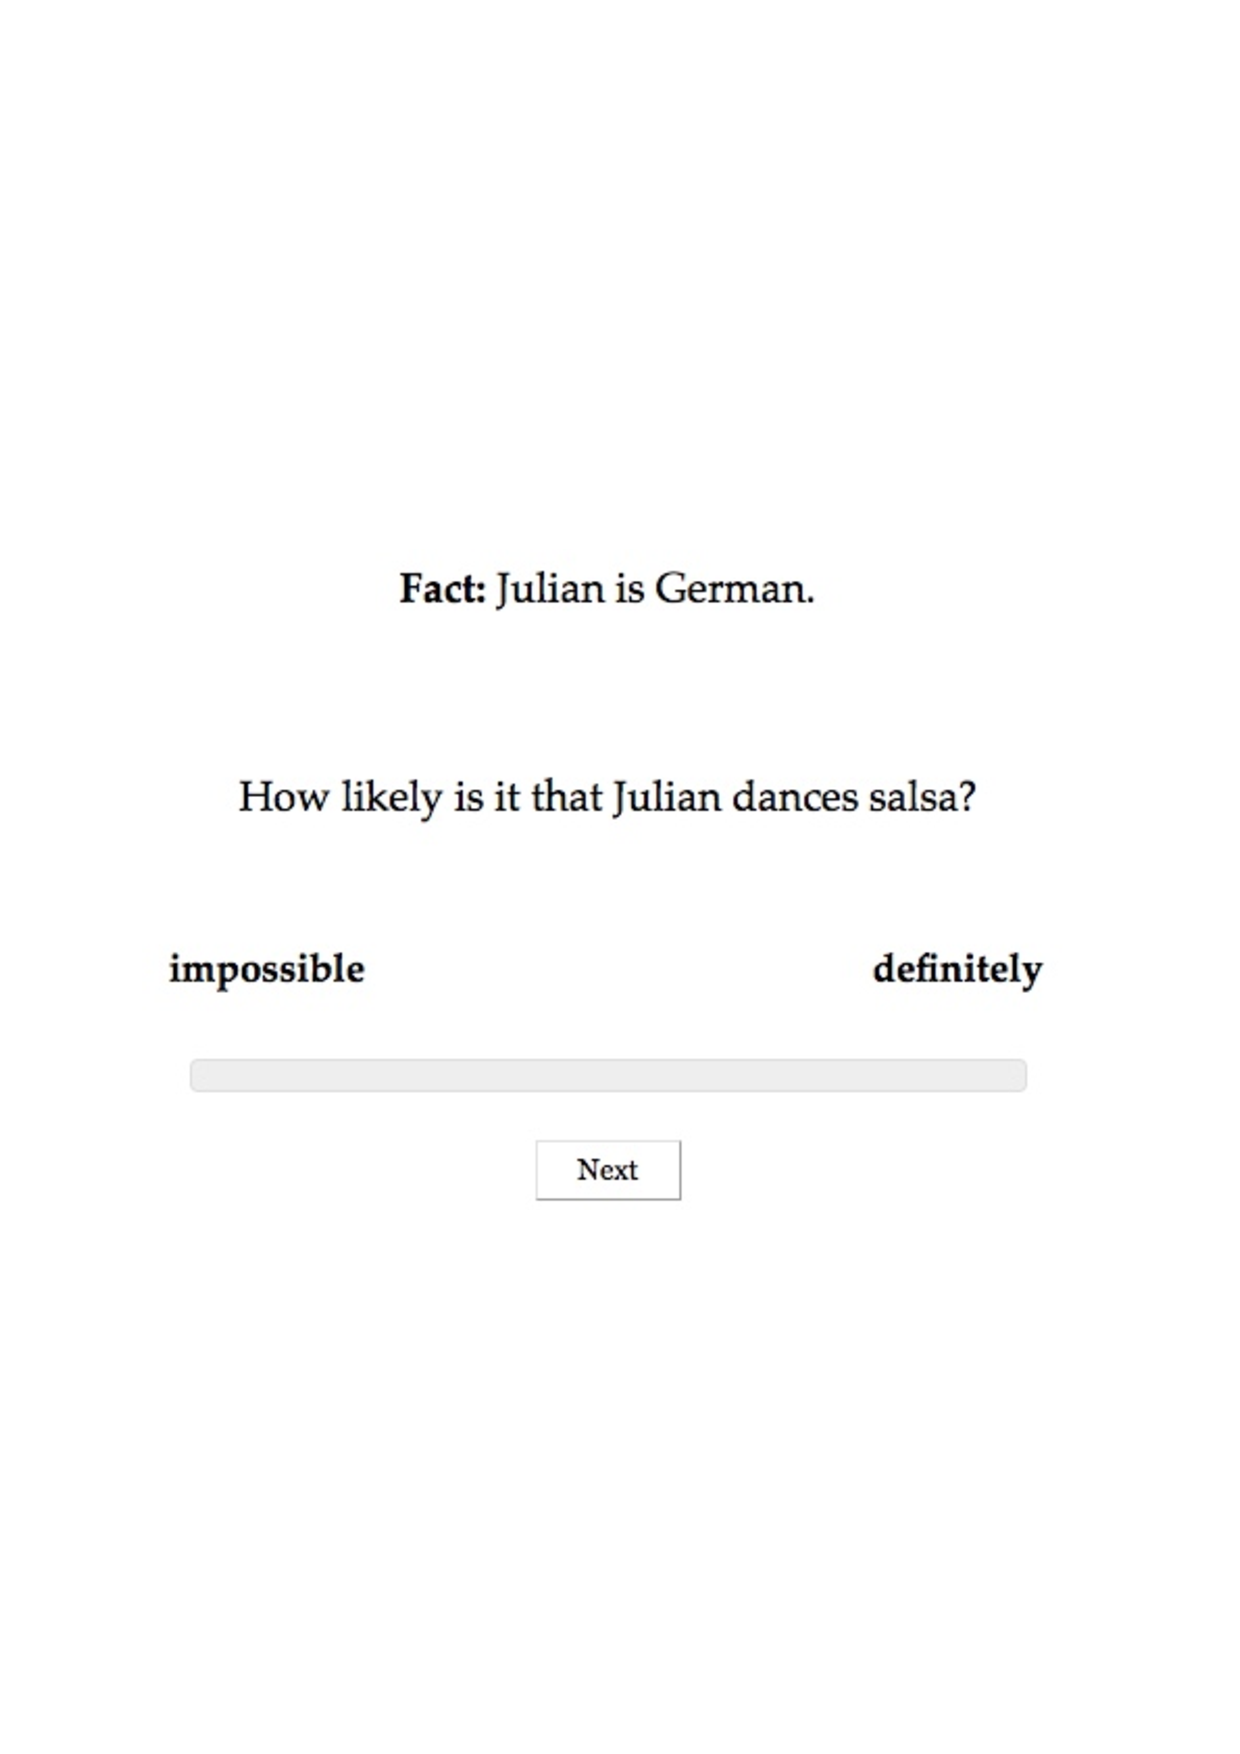
\includegraphics[width=7.55cm]{figures/exp1-prior-trial}}
\caption{Target trial in prior block.}\label{fig-exp1-prior}
\end{subfigure}%
\begin{subfigure}[t]{0.5\textwidth}
\centering
\fbox{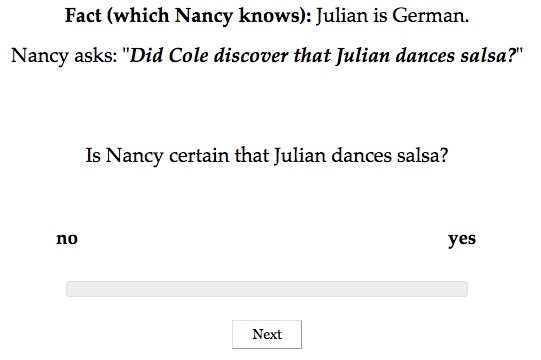
\includegraphics[width=7.9cm]{figures/exp1-projection-trial}} 
\caption{Target trial in projection block.}\label{fig-exp1-projection}
 \end{subfigure}
 \par\bigskip
\begin{subfigure}[t]{1\textwidth}
        \centering
       \fbox{\begin{minipage}{15cm}{\em acknowledge, admit, announce, be annoyed, be right, confess, confirm, demonstrate, discover, establish, hear, inform, know, pretend, prove, reveal, say, see, suggest, think. }\end{minipage}}
\caption{20 clause-embedding predicates.}\label{fig-exp1-preds}
\end{subfigure}
\par\bigskip
\begin{subfigure}[t]{0.5\textwidth}
\centering
\fbox{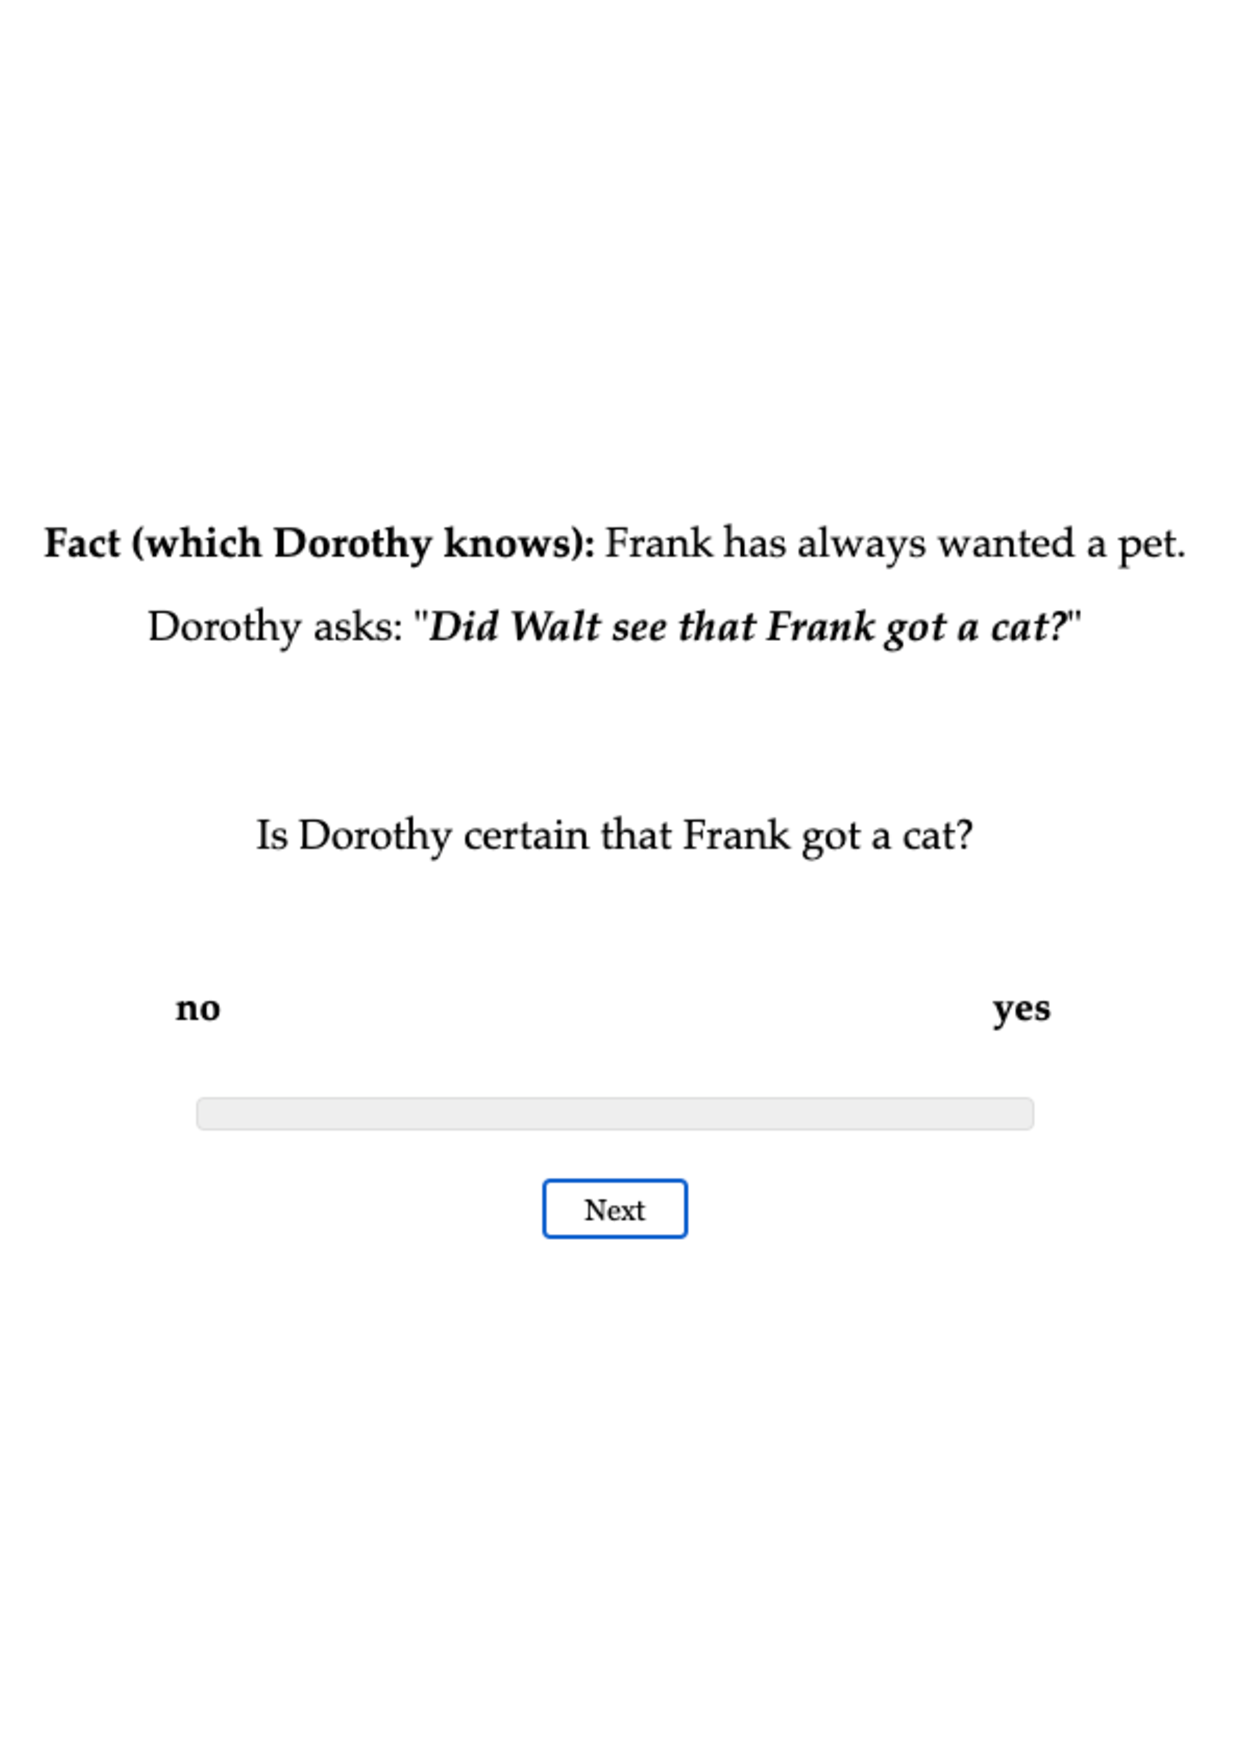
\includegraphics[height=5.4cm,width=7.9cm]{figures/exp1-projection-control}} 
\caption{Control trial in projection block.}\label{fig-exp1-projection-control}
 \end{subfigure}%
\begin{subfigure}[t]{0.5\textwidth}
        \centering
\fbox{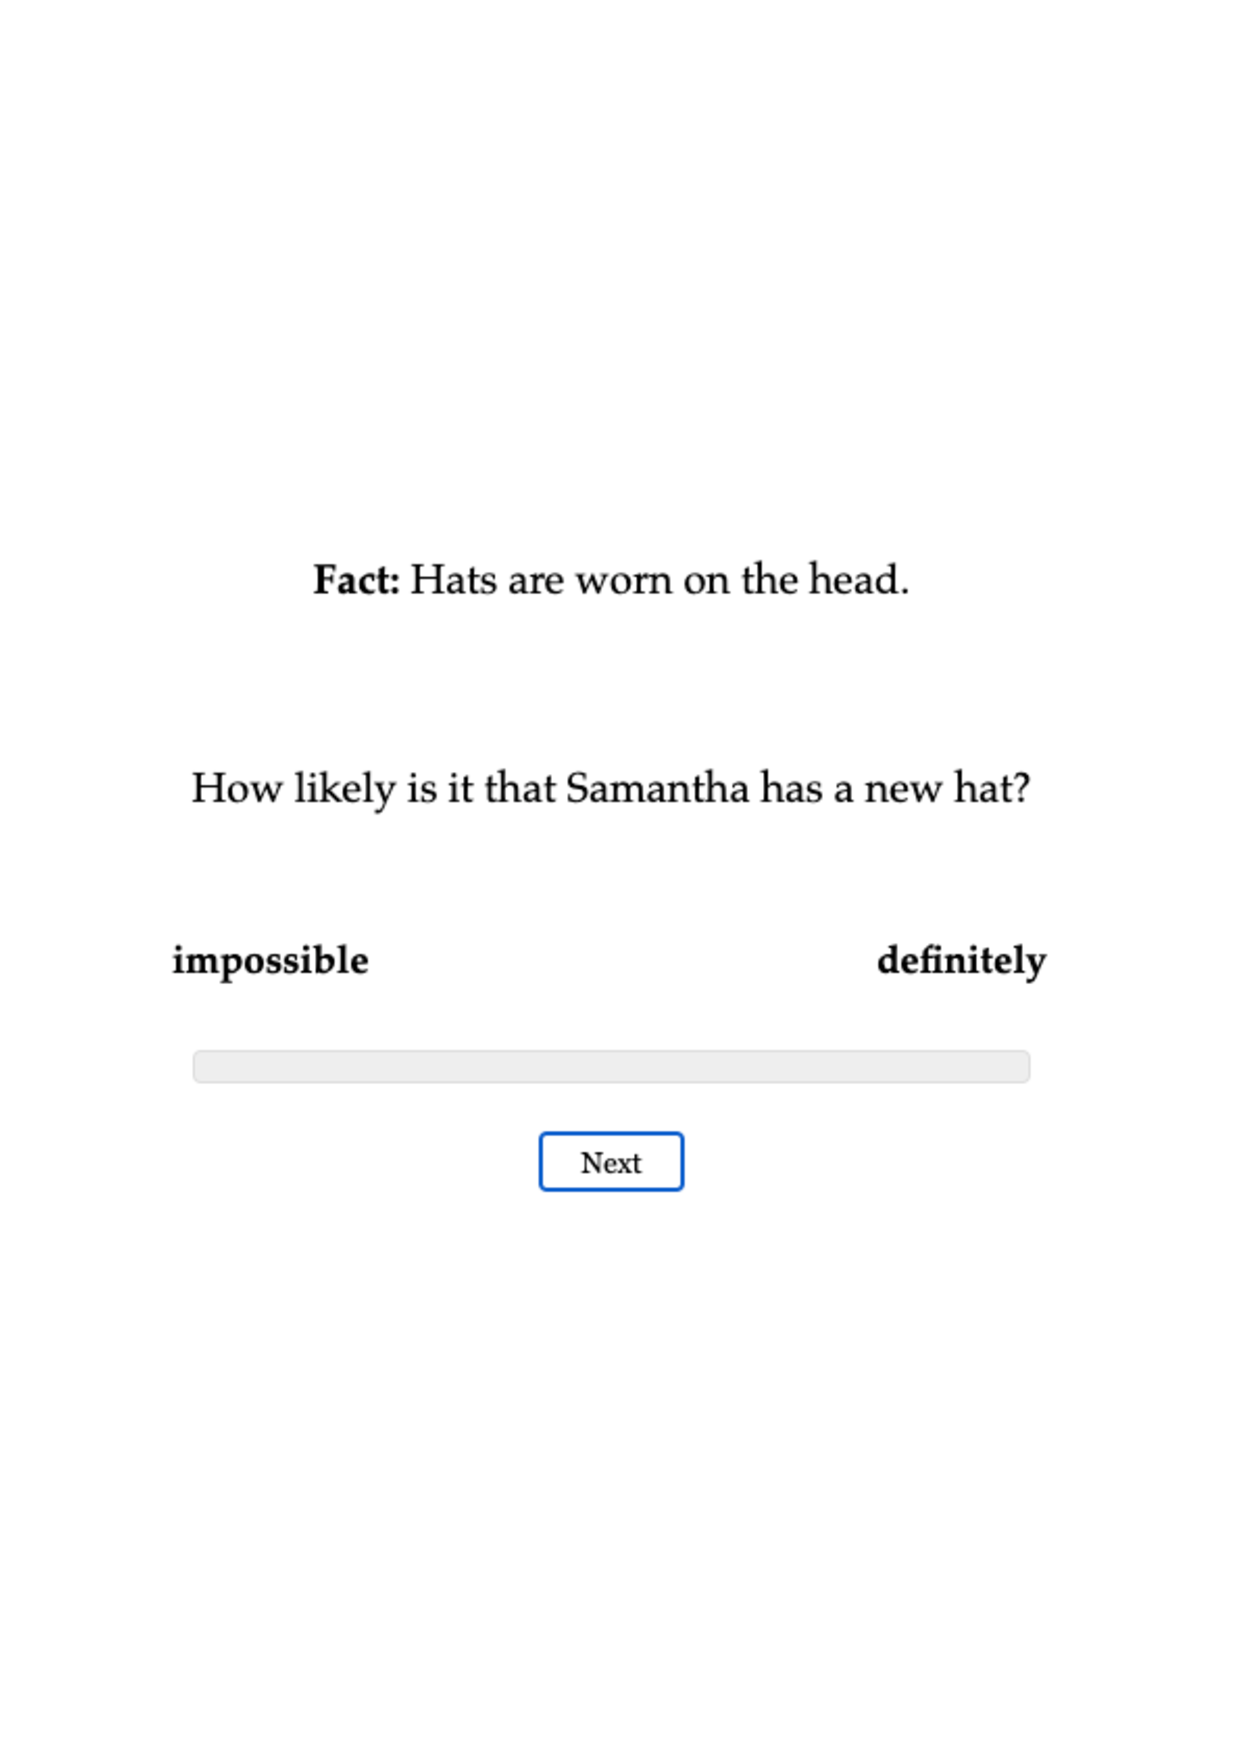
\includegraphics[height=5.4cm,width=7.6cm]{figures/exp1-prior-filler}}
\caption{Filler trial in prior block.}\label{fig-exp1-prior-filler}
\end{subfigure}


\caption{Sample trials and 20 clause-embedding predicates in Exp.~1.}
\end{figure}

After completing the experiment, participants filled out a short optional demographic survey. To encourage truthful responses, participants were told that they would be paid no matter what answers they gave in the survey.

\paragraph{Data exclusion} Data was excluded based on self-declared non-native speaker status and other criteria given in Supplement \ref{a-exclusion}, leaving 7436 data points from 286 participants to be analyzed (ages 18-82; median: 35.5; 116 female, 186 male, 1 other, 1 undeclared).

\subsection{Results and discussion}

\jt{Ick! Lonely section 2.1. But if we turn this into paragraph, then what to do with the next two paragraphs?}

\paragraph{Prior beliefs.}  \figref{f-prior} shows the mean prior probabilities of the 20 contents by fact. Each content's mean prior probability  was rated as higher when it was presented with its higher probability fact than when it was presented with its lower probability fact ($\beta$ = 0.45, $SE$ = 0.01, $t$ = 31.12, $p$ $<$ .0001), as assessed in a mixed-effects linear regression predicting slider rating from dummy-coded fact type (reference level: `lower probability') and random by-item and by-participant intercepts and slopes for fact type.\footnote{All analyses were conducted in R \cite{R} using the \texttt{lme4} package \cite{lme4}.} This suggests that the manipulation of the prior probability of the 20 contents was successful. 

\begin{figure}[h!]
\centering
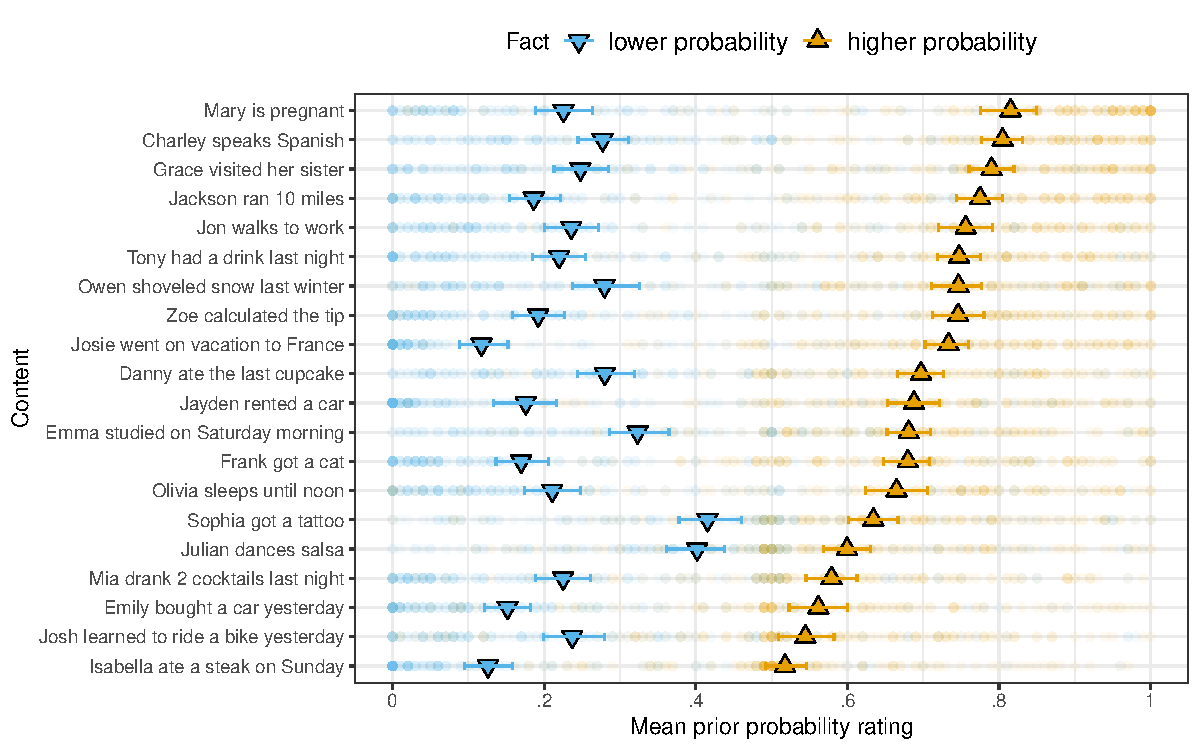
\includegraphics[width=.7\paperwidth]{../../results/9-prior-projection/graphs/prior-ratings}

\caption{Mean prior probability by content and fact in Exp.~1. Error bars indicate 95\% bootstrapped confidence intervals. Transparent dots indicate individual participant ratings.} 
\label{f-prior}
\end{figure}

\paragraph{Do prior beliefs modulate projection?}  \figref{f-projection-mean} shows the mean certainty ratings for the CCs by  predicate and by fact, as well as the mean certainty rating for the main clause controls (abbreviated `MC'). The mean certainty ratings were higher for contents  presented with higher probability facts than for contents presented with lower probability facts ($\beta$ = 0.14, $SE$ = 0.01, $t$ = 12.24, $p$ $<$ .0001), as assessed by a mixed effects linear regression predicting certainty ratings from dummy-coded fact type (reference level: `lower probability') and random by-item and by-participant intercepts and slopes for fact type.  This result, which holds for all 20 clause-embedding predicates, suggests that participants' prior beliefs about content probability systematically modulated the extent to which they take the speaker to be committed to that content.

\begin{figure}[h!]
\centering

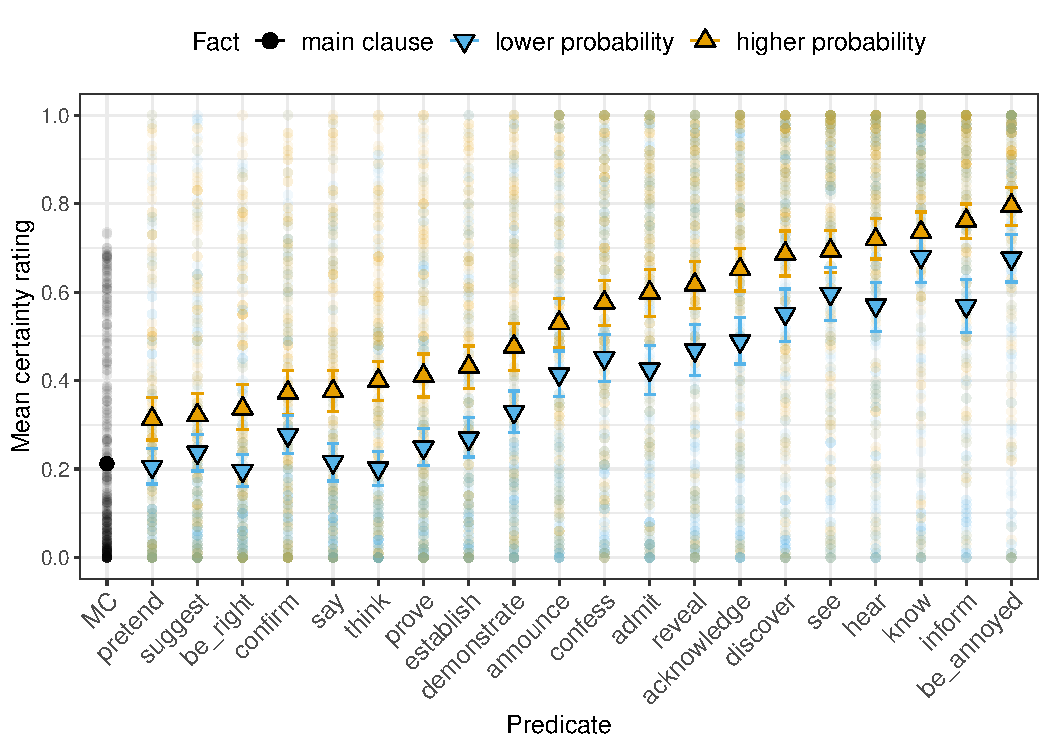
\includegraphics[width=.7\paperwidth]{../../results/9-prior-projection/graphs/means-projectivity-by-predicate-and-prior}

\caption{Mean certainty ratings by predicate and prior probability of the content of the complement in Exp.~1. Error bars indicate 95\% bootstrapped confidence intervals. Light dots indicate participants' ratings.} 
\label{f-projection-mean}
\end{figure}

We also replicated \citeA{tonhauser-degen-factive}'s result of by-predicate variation in the projection of the CC: for instance, the CC of {\em be annoyed} was more projective than that of {\em discover}, which in turn was more projective than that of {\em announce}. The Spearman rank correlation between the mean certainty ratings in Exp.~1 (collapsing over facts) and \citepos{tonhauser-degen-factive} Exp.~1a is .991; see Supplement \ref{a-comparison} for a visualization. Exp.~1 thereby also provides further evidence for the systematic influence of the predicate on projection, but crucially the effect of the prior was observable independently of predicate.

Closer inspection of  \figref{f-prior} reveals by-participant variability in prior probability ratings. This means that individual participants' prior beliefs may not align with the prior probability classification assumed in  \figref{f-projection-mean}. For example, given a particular content (e.g., that Julian dances salsa), it is possible that one participant's prior probability rating was lower than that of another participant, even though the first participant was presented with the higher probability fact (Julian is Cuban) and the second one with the lower probability fact (Julian is German). \figref{f-projection} shows participants' certainty ratings by their individual prior probability ratings. %(The color coding here merely represents the type of fact the participant was presented with. No classification is imposed.) The linear smoothers suggest a positive correlation for each predicate between prior probability and certainty ratings such that contents with higher prior probability ratings receive higher certainty ratings. 
To investigate whether prior beliefs modulate projection at the by-participant level,  we conducted the same mixed-effects analysis reported above,\jt{but above we're predicting mean certainty ratings and here were predicting individual certainty ratings, no?} but used participants' individual prior probability ratings as the fixed effect prior predictor. Again, higher-prior-probability CCs were more likely to project ($\beta$ = 0.28, $SE$ = 0.02, $t$ = 13.85, $p$ $<$ .0001). This  suggests that prior probability influences projection even at the by-participant level. In fact, a Bayesian Information Criterion (BIC) model comparison  revealed that the individual-level model better captured the variance in the data (group-level model BIC: 2654; participant-level model BIC: 2291), suggesting that individual listeners' prior beliefs systematically modulate the extent to which they take the speaker to be committed to a content: the more they believe it, the more they take the speaker to believe it.

\begin{figure}[h!]
\centering

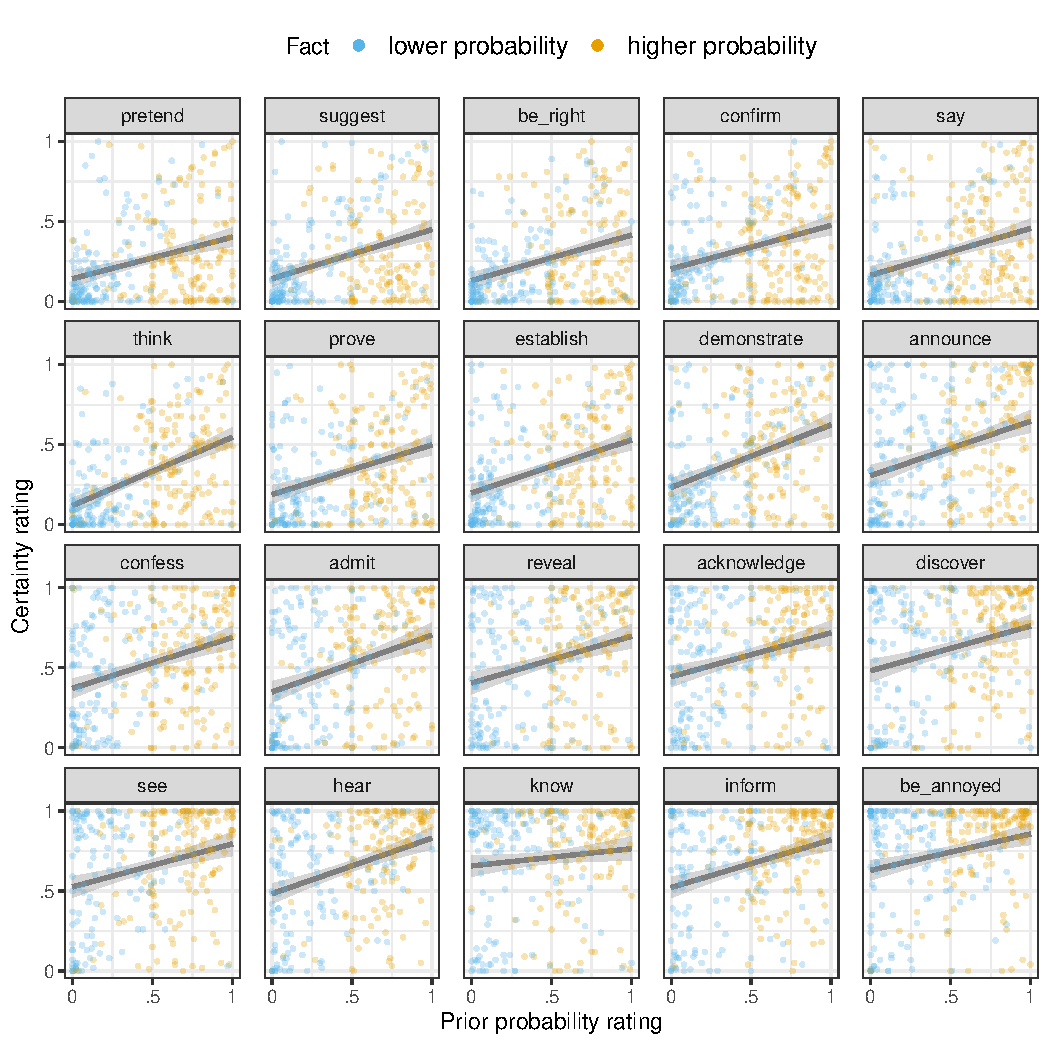
\includegraphics[width=.7\paperwidth]{../../results/9-prior-projection/graphs/projection-by-prior}

\caption{Certainty ratings by prior probability ratings by predicate in Exp.~1. Linear smoothers with 95\% confidence intervals are overlaid.}
\label{f-projection}
\end{figure}

%\newpage
%
%The qualitative observations about the relations between prior probability, clause-embedding predicate and projection were borne out statistically. We fitted a Bayesian mixed effects Beta regression model  with weakly informative priors using the \verb|brms| \cite{buerkner2017}  package in R \cite{R} on the target data (5,720 data points). The model predicted the certainty ratings from a fixed effect of prior probability and included the maximal random effects structure justified by the design, namely random by-participant and by-item intercepts (where an item is a combination of a predicate and a complement clause). A Beta regression model estimates the mean of the outcome distribution (like a linear regression model).\footnote{Beta regression models also estimate a second parameter, namely the precision, which is a measure of dispersion: the greater the precision, the more concentrated the ratings are around the mean. In this paper, we rely on the estimated mean to identify whether prior probability predicts projection. Both the estimated mean and precision are reported in the full model output table in Supplement \ref{modeldetails}.} We thus obtain a 95\% credible interval for \jt{the mean effect of prior probability on certainty?}. Supplement \ref{modeldetails} motivates the use of Beta regression over linear regression, provides a brief primer on how to interpret Bayesian mixed effects Beta regression models, and reports the full model output.
%
%\jt{We need to report two models here: predicting projection from prior at by-participant level, but also predicting mean projection from mean prior, to allow for comparison to Exps.~2}
%
%\jt{According to the Beta regression model, the estimated mean for each predicate was higher when....} 


The results of Exp.~1 provide empirical support for the hypothesis that higher prior probability content is more likely to project. It is possible, however, that the within-participant design resulted in participants' responses on either block influencing their responses on the other block. To mitigate against this possibility, we conducted Exps.~2, where prior probability and projection ratings were collected from different populations.  

\section{Experiments 2}\label{s3}

Exps.~2a and 2b measured the prior probability and the projection of the 20 contents of Exp.~1, respectively.

\subsection{Methods}

%Exp 2a: November 13, 2017
%Exp 2b: November 28, 2017

\paragraph{Participants} Participants with U.S.\ IP addresses and at least 99\% of previous HITs approved were recruited on Amazon's Mechanical Turk platform. The 95 participants in Exp.~2a (ages: 21-75, median: 33; 45 female, 50 male) were paid 55 cents. The 300 participants in Exp.~2b (ages: 21-72, median: 36; 145 female, 154 male, 1 undeclared) were paid 85 cents.\footnote{28 participants took both experiments. Given that the experiments were run two weeks apart (Exp.~2a on November 13, 2017 and Exp.~2b on November 28, 2017, it is unlikely that these 28 participants' prior ratings influenced their projection ratings.}

\paragraph{Materials and procedures} The 40 target stimuli of Exp.~2a were identical to those of the prior block of Exp.~1. Each participants saw the two control stimuli in (\ref{control2}), which were included to assess attention to the task. We expected high prior probability ratings for (\ref{control2}a) and low ones for (\ref{control2}b). 

\begin{exe}
\ex\label{control2}
\begin{xlist}
\ex {\bf Fact:} Barry lives in Germany. \\ How likely is it that Barry lives in Europe?
\ex {\bf Fact:} Tammy is a rabbit. \\ How likely is it that Tammy speaks Italian and Greek?
\end{xlist}
\end{exe}
The materials of Exp.~2b were identical to those of the projection block of Exp.~1. Trial order in both experiments was random. The procedures of Exps.~2a and 2b were identical to those of the prior and projection blocks of Exp.~1, respectively.

\paragraph{Data exclusion} We excluded data based on the criteria given in Supplement \ref{a-exclusion}, leaving data from 75 participants to be analyzed in Exp.~2a (ages 21-75; median: 35; 34 female, 41 male) and from 266 participants in Exp.~2b (ages 21-72; median: 36; 129 female, 136 male, 1 undeclared).

\subsection{Results}

Exp.~2a replicated the prior probability manipulation of Exp.~1.  \figref{f-prior-comparison} plots the mean prior probability ratings in Exp.~2a against those of Exp.~1. The Spearman rank correlation was high, at .977. For a visualization of the by-content prior ratings see Supplement \ref{a-exp2}.

\begin{figure}[h!]
\centering

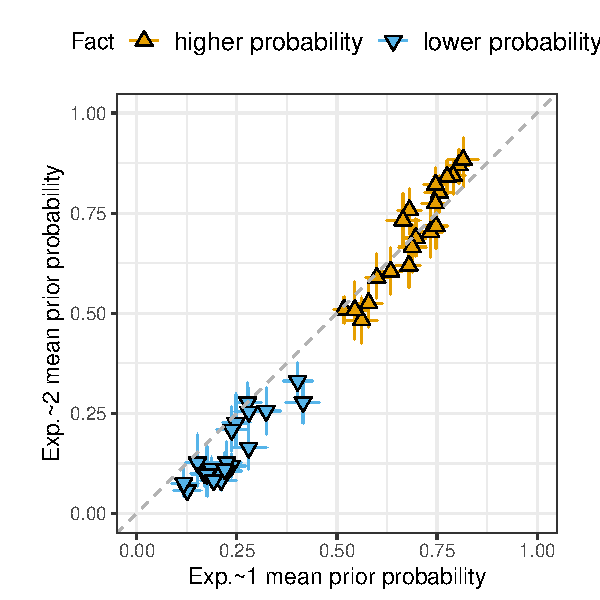
\includegraphics[width=.4\paperwidth]{../../results/1-prior/graphs/prior-probability-comparison-exp1-exp2}

\caption{Mean prior probability ratings in Exp.~2a against those of Exp.~1. Error bars indicate 95\% bootstrapped confidence intervals. The dotted line indicates \jt{what?}.}
\label{f-prior-comparison}
\end{figure}

Exp.~2b replicated the critical result of Exp.~1, that prior probability influences projection.\footnote{Exp.~2b also replicated \citepos{tonhauser-degen-factive} result that there is by-predicate variation in the projection of the content of the complement; see Supplement \ref{a-comparison}.}  \figref{f-projection-mean-2b} shows that mean certainty ratings in Exp.~2b were higher for contents presented with higher probability facts than for contents presented with lower probability facts.

\begin{figure}[h!]
\centering

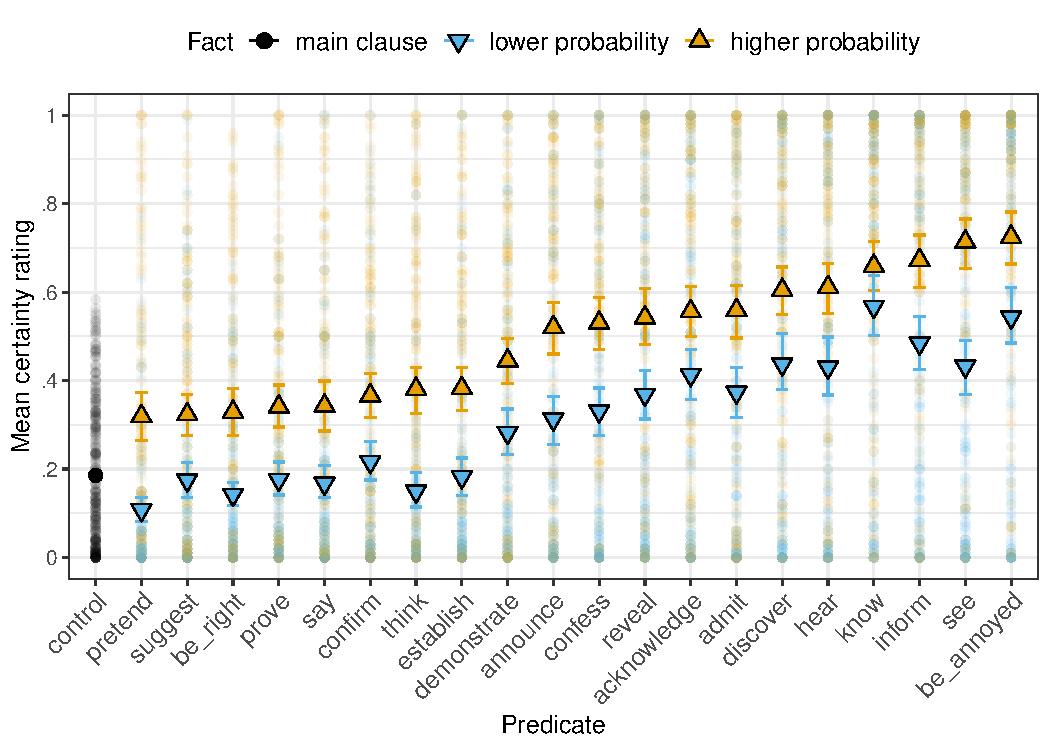
\includegraphics[width=.7\paperwidth]{../../results/3-projectivity/graphs/means-projectivity-by-predicate-and-prior}

\caption{Mean certainty ratings by predicate and prior probability of the content of the complement in Exp.~2b. Error bars indicate 95\% bootstrapped confidence intervals. Light dots indicate participants' ratings.} 
\label{f-projection-mean-2b}
\end{figure}


\jt{report models predicting a) projection mean Exp 2b from prior mean Exp 2b, b) projection mean Exp 1 from prior mean Exp 2b, and c) projection mean Exp 2b from prior mean Exp 1). USE COHENS D?} These results suggest that the result of Exp.~1 is not an artifact of the within-participant design of Exp.~1.

\subsection{Discussion}

\jt{need to smoothe transition}

These results confirm \citepos{mahler2020} results and expand on them in several ways. First, while \citeNP{mahler2020} manipulated only the political party affiliation of the speaker, the manipulation in Exp.~1 relied on 20 distinct properties of the individuals denoted by the subjects of the 20 clauses (e.g., whether Julian is more likely to dance salsa if he is German or Cuban, or whether Zoe is more likely to have calculated the tip, if she is 5 years old or a math major). Thus, the result of Exp.~1 suggests a general effect of prior probability on projection.\footnote{None of our prior probability manipulations relied on gender stereotypes because we only became aware of \citeNP{lorson2018} after running Exp.~2.}

Second, while \citeNP{mahler2020} observed an influence of prior probability of the projection of the CCs of two classes of predicates (so-called factive and non-factive predicates), Exp.~1 observed such an influence for the CCs of 20 predicates. Thus, the result of Exp.~1 supports the assumption that the effect of prior probability on projection is more general than was suggested in \citeNP{mahler2020}. In fact, the results of Exp.~1 motivate the hypothesis that prior probability influences projection across the set of English clause-embedding predicates. Finally, prior probability and projection were measured in a within-participant design in Exp.~1, in contrast to \citeposs{mahler2020} experiment, which only measured projection.  Exp.~1 thus supports the claim that projection is influenced not only by the average prior probability of content but also by the prior probability that individual listeners assign to content. This result suggests that by-participant variability in projection experiments (see, e.g., \citeNP{tbd-variability,tonhauser-degen-factive}) may be due to participants assigning different prior probabilities to the contents under investigation. 

\section{Concluding remarks}\label{s4}

This paper provided empirical support for \citetpos{stevens-etal2017} and \citetpos{tbd-variability} hypothesis that listeners' beliefs about utterance content influence their inferences about speaker commitment to that content. A pressing question for future research is how prior probabilities interact with other factors that have been shown to influence projection, such as the content's discourse status and utterance prosody. On the theoretical side, our result motivates the development of projection analyses that predict the influence of prior probability on the projection of the content of English clause-embedding predicates. Analyses currently on the market do not predict the results of our experiments  because they are limited to subsets of clause-embedding predicates, like factive ones (e.g., \citeNP{heim83,vds92,abrusan2011,abrusan2016,romoli2015,best-question}).


% Brief research report: up to 4,000 words
% remove comment from next line for word count (word count includes abstract, main body and figure captions, but not references or supplement)
%\end{document}

%\bibliographystyle{../cslipubs-natbib}
\bibliographystyle{apacite}
%
%
%\setlength{\bibleftmargin}{.125in}
%\setlength{\bibindent}{-\bibleftmargin}
\bibliography{../../bibliography}

\newpage

\appendix

\setcounter{table}{0}
\renewcommand{\thetable}{A\arabic{table}}

\setcounter{figure}{0}
\renewcommand{\thefigure}{A\arabic{figure}}

\section*{Supplemental material for {\em Prior probability predicts projection}}

\section{Experiment 1: Target and control stimuli}\label{a-stim}

This list gives the 20 clauses of the target stimuli with the lower and higher probability facts, respectively:

\begin{enumerate}[leftmargin=4ex,itemsep=-2pt]
\item Mary is pregnant. Facts: Mary is a middle school student / Mary is taking a prenatal yoga class
\item Josie went on vacation to France. Facts:  Josie doesn't have a passport / Josie loves France 
\item Emma studied on Saturday morning. Facts: Emma is in first grade / Emma is in law school 
\item Olivia sleeps until noon. Facts: Olivia has two small children / Olivia works the third shift
\item Sophia got a tattoo. Facts: Sophia is a high end fashion model / Sophia is a hipster
\item Mia drank 2 cocktails last night. Facts: Mia is a nun / Mia is a college student
\item Isabella ate a steak on Sunday. Facts: Isabella is a vegetarian / Isabella is from Argentina
\item Emily bought a car yesterday. Facts: Emily never has any money / Emily has been saving for a year
\item Grace visited her sister. Facts: Grace hates her sister / Grace loves her sister
\item Zoe calculated the tip. Facts: Zoe is 5 years old / Zoe is a math major
\item Danny ate the last cupcake. Facts: Danny is a diabetic / Danny loves cake
\item Frank got a cat. Facts: Frank is allergic to cats / Frank has always wanted a pet
\item Jackson ran 10 miles. Facts: Jackson is obese / Jackson is training for a marathon
\item Jayden rented a car. Facts: Jayden doesn't have a driver's license / Jayden's car is in the shop
\item Tony had a drink last night. Facts: Tony has been sober for 20 years / Tony really likes to party with his friends
\item Josh learned to ride a bike yesterday. Facts: Josh is a 75-year old man / Josh is a 5-year old boy
\item Owen shoveled snow last winter. Facts: Owen lives in New Orleans / Owen lives in Chicago
\item Julian dances salsa. Facts: Julian is German / Julian is Cuban
\item Jon walks to work. Facts: Jon lives 10 miles away from work / Jon lives 2 blocks away from work
\item Charley speaks Spanish. Facts: Charley lives in Korea / Charley lives in Mexico
\end{enumerate}

In the target stimuli of the projection block of Exp.~1, eventive predicates, like {\em discover} and {\em hear}, were realized in the past tense and stative predicates, like {\em know} and {\em be annoyed}, were realized in the present tense. The direct object of {\em inform} was realized by the proper name {\em Sam}. The subject of the clause-embedding predicate and the speaker of the target stimuli were realized by a proper name. 

The following list gives the six clauses that were used in the control and filler stimuli of Exp.~1, with their facts. In the prior block, these six clauses were embedded under {\em How likely is it that\ldots?}. The projection block featured polar questions variants of the clauses.

\begin{enumerate}[leftmargin=3ex,itemsep=-2pt]
\ex Zack is coming to the meeting tomorrow. Fact: Zack is a member of the golf club. 

\ex Mary's aunt is sick. Fact: Mary visited her aunt on Sunday. 

\ex Todd played football in high school. Fact: Todd goes to the gym 3 times a week. 

\ex Vanessa is good at math. Fact: Vanessa won a prize at school. 

\ex Madison had a baby. Fact: Trish sent Madison a card. 

\ex Hendrick's car was expensive. Fact: Hendrick just bought a car. 
\end{enumerate}

\section{Data exclusion}\label{a-exclusion}

Table \ref{f-exclusion} presents how many participants' data were excluded from the analyses based on the exclusion criteria. The first column records the experiment, the second (`recruited') how many participants were recruited, and the final column (`remaining') how many participants' data entered the analysis. The `Exclusion criteria' columns show how many participants' data were excluded based on the two exclusion criteria: 

\begin{itemize}[topsep = -1ex,itemsep=-2pt]

%\item `multiple': Due to an experimental glitch, some participants participated in Exps.~1b, 2b or 3b more than once. Of these participants, we only analyzed the data from the first time they participated.

\item `language': Participants' data were excluded if they did not self-identify as native speakers of American English.

\item `controls': In Exps.~1 and 2b, participants' data were excluded if their response mean on the 6 control items was more than 2 sd above the group mean. In Exp.~2a, participants' data were excluded if their response mean was more than 2 sd below the group mean of the control in (\ref{control}a) or more than 2 sd above the group mean of the control in (\ref{control}b).

%\item `variance': Participants' data were excluded if they always selected roughly the same point on the response scale, that is, if the variance of their response distribution was more than 2 sd below the group mean variance. \jt{did we do variance or not? if not, why not?}

\end{itemize}

% exp 1 (prior, projection)
%Prior to analysis, the data from 3 participants who did not self-identify as native speakers of American English were excluded. To assess whether the remaining 297 participants attended to the task, we inspected their responses to the control stimuli. We excluded the data from 11 participants whose response means were more than 2 standard deviations above the group mean. The data from 286 participants (ages 18-82; median: 35.5; 116 female, 186 male, 1 other, 1 undeclared) were analyzed.

% exp 2a (prior):
%Prior to analysis, the data from 8 participants who did not self-identify as native speakers of American English were excluded. To assess whether the remaining 87 participants attended to the task, we inspected their responses to the 2 control stimuli. The response means of 12 participants were more than 2 standard deviations below the group mean of the control in (\ref{control}a) or more than 2 standard deviations above the group mean of the control in (\ref{control}b). We excluded the data from these participants, leaving data from 75 participants (ages 21-75; median: 35; 34 female, 41 male).

% exp 2b (projection):
%Prior to analysis, the data from 23 participants who did not self-identify as native speakers of American English were excluded. To assess whether the remaining 277 participants attended to the task, we inspected their responses to the 6 control stimuli. There were 11 participants whose response means were more than 2 standard deviations above the group mean. We excluded the data from these participants, too, leaving data from 266 participants (ages 21-72; median: 36; 129 female, 136 male, 1 undeclared).

\begin{table}[h!]
\centering
\begin{tabular}{l r | r r | r}
&  & \multicolumn{2}{c|}{Exclusion criteria} &  \\ 
&  recruited  & language & controls & remaining \\ 
\hline
Exp.~1 & 300 & 3 & 11 & 286 \\
Exp.~2a & 95 & 8 & 12 & 75 \\
Exp.~2b & 300 & 23 & 11 & 266 \\
\end{tabular}
\caption{Data exclusion in Exps.~1 and 2}\label{f-exclusion}
\end{table} 

\section{Model details for Experiments 1 and 2}\label{modeldetails}

\jt{do we need this for this journal? if not, cool, let's delete. if yes, needs to be adjusted.}

This supplement provides details on the data analysis conducted for Exps.~1, 2, and 3. We first motivate the use of Beta regression rather than linear regression in Exps.~1a, 2a, and 3a (section \ref{a-motivation}) and then provide a brief primer on how to interpret Bayesian mixed effects Beta regression models (section \ref{a-primer}). We then report the model outputs for Exps.~1, 2, and 3 (section \ref{a-mo}).

\subsection{Motivation for using Bayesian mixed effects Beta regression}\label{a-motivation}

There are three separate pieces to motivate: the use of \emph{mixed effects}, the use of a \emph{Bayesian} rather than \emph{frequentist} models, and the use of \emph{Beta regression} rather than \emph{linear regression}. 

\textbf{Using mixed effects} refers to the practice of modeling the outcome variable, here slider ratings or proportions of `yes' ratings, as a function of not just fixed effects of interest (i.e., predicate) but also as the result of possible random variability that is not of theoretical interest (e.g., random by-participant or by-item variability). This is standard practice in psycholinguistic studies and allows the researcher to trust that any observed effects of theoretical interest are true average effects rather than the result of idiosyncratic behavior (e.g., of participants or items). This is also the motivation for using mixed effects in Exps.~1b, 2b, and 3b.

\textbf{Using Bayesian models} rather than frequentist models is increasingly becoming the norm in psycholinguistic studies as computational power has increased and running Bayesian models has become more accessible with the introduction of R packages such as \verb|brms| \cite{buerkner2017}. The presence of an effect in frequentist models is evaluated by checking whether the {\em p-}value is smaller than $.05$, where the {\em p-}value is defined as the probability of obtaining data that is as skewed or more skewed than the observed data if the null-hypothesis was true, i.e., if the hypothesized effect was absent. Parameter estimates in frequentist models are obtained via maximum-likelihood techniques, i.e., by estimating the parameter values that maximize the probability of observing the data. Bayesian models, by contrast, return a full posterior distribution over parameter values that take into account not just the probability of the data under the parameter values, but also the prior probability of parameter values. In order to evaluate the evidence for an effect of a predictor of interest, one can report 95\% credible intervals and the posterior probability $P(\beta < 0)$ or $P(\beta > 0)$ that the predictor coefficient $\beta$ is either lower or greater than zero, depending on the direction of the expected effect. A 95\% credible interval (CI) demarcates the range of values that comprise 95\% of probability mass of the posterior beliefs such that no value inside the CI has a lower probability than any point outside it \cite{Jaynes1976, Morey2016}. There is substantial evidence for an effect if zero is (by a reasonably clear margin) not included in the 95\% CI and $P(\beta > 0)$ or $P(\beta < 0)$ is close to zero or one. Posterior probabilities indicate the probability that the parameter has a certain value, given the data and model -- these probabilities are thus \emph{not} frequentist {\em p-}values. In order to present statistics as close to widely used frequentist practices, and following \citeNP{Nicenboim2016}, we defined an inferential criterion that seems familiar (95\%), but the strength of evidence should not be taken as having clear cut-off points (such as in a null-hypothesis significance testing framework).

\textbf{Using Beta regression} rather than linear regression was motivated by the violation of two of the  assumptions of linear regression: first, that residuals be normally distributed (where ``residuals'' refers to the residual error for each data point after fitting the model), and second, that the error term exhibit homoscedasticity (that it be roughly the same across different conditions). Slider ratings data has the property of being bounded by its endpoints (which we code as 0 and 1, respectively). This often leads to ``bunching'' behavior at the endpoints (see  \figref{fig:bunch} for the distribution of raw ratings in Exps.~1a, 2a, and 3a). 


\begin{figure}[h!]
\begin{subfigure}{.33\textwidth}
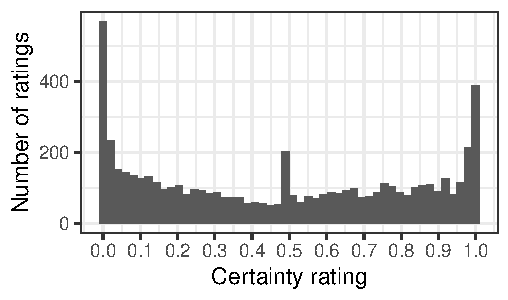
\includegraphics[width=\textwidth]{../../results/9-prior-projection/graphs/bunching-projection}
\caption{Exp.~1 certainty ratings.}
\label{fig:exp1araw}
\end{subfigure}
\begin{subfigure}{.33\textwidth}
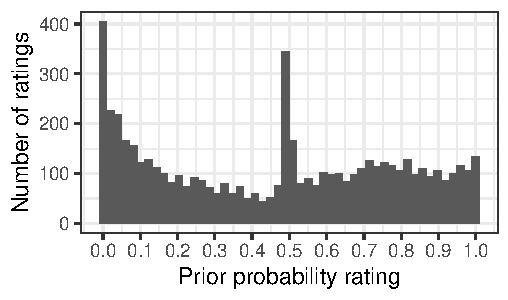
\includegraphics[width=\textwidth]{../../results/9-prior-projection/graphs/bunching-prior}
\caption{Exp.~1 prior ratings.}
\label{fig:exp2araw}
\end{subfigure}
\begin{subfigure}{.33\textwidth}
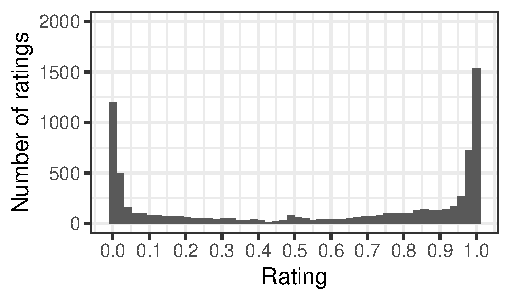
\includegraphics[width=\textwidth]{../../results/2-veridicality2/graphs/bunching}
\caption{Exp.~2 prior ratings.}
\label{fig:exp3araw}
\end{subfigure}
\caption{Histograms of raw slider ratings in Exps.~1 and 2.}
\label{fig:bunch}
\end{figure}

This ``bunching'' behavior, in turn, can lead to the violation of both of the above assumptions of linear regression. 
Intuitively, these assumptions are violated because conditions that elicit ratings closer to endpoints necessarily have a compressed variance; consequently, a condition's mean and its variance are not independent. Beta regression is useful here because it allows for modeling an arbitrarily distributed outcome variable in the $[$0,1$]$ interval. The Beta distribution is characterized by two parameters, one capturing the mean $\mu$ of the distribution and one capturing its precision $\phi$, a measure of dispersion. The greater the precision, the more concentrated the values are around the mean, i.e., the lower the variance of the distribution.  We follow \citeA{smithson2006} in modeling $\mu$ and $\phi$ separately for each predictor. That is, we allow each predictor to affect both the mean and the precision of the outcome variable's distribution. 

\subsection{Coding choices and interpreting model output}\label{a-primer}

The outcome variable in Exps.~1a, 2a and 3a (slider ratings) contained the values 0 and 1, which Beta regression is undefined for. We therefore applied a common transformation to ratings before the main analysis that rescales values $y$ to fall in the open unit interval (0,1)  \cite{smithson2006}. First, we apply $y' = (y-a)/(b-a)$, where $b$ is the highest possible slider rating and $a$ is the smallest possible slider rating. The range is then compressed to not include 0 and 1 by applying $y'' = [y'(N-1) + 1/2]/N$, where $N$ is the total number of observations.

The mean parameter $\mu$ is modeled via a logit link function (default for Beta regression in \verb|brms|), though other links that squeeze $\mu$ into the $[$0,1$]$ interval are possible. The dispersion parameter $\phi$ is modeled via a log link, which ensures that values of $\phi$ are strictly positive, which is necessary because a variance cannot be negative. 

We allowed both $\mu$ and $\phi$ to vary as a function of predicate, with reference level set to main clause control in Exp.~1a, entailing control in Exp.~2a and contradictory control in Exp.~3a. We also allowed random intercept adjustments to each parameter by participant and by item, where item was defined as a unique combination of a predicate and a complement clause. Four chains converged after 2000 iterations each (warmup = 1000, \(\hat{R}=1\) for all estimated parameters) with a target acceptance rate of .95 and a maximum treedepth of 15.

\subsection{Model outputs for Experiments 1, 2 and 3}\label{a-mo}

The three tables in this section show the model outputs for Exps.~1, 2 and 3, respectively: Table \ref{tab:exp1modelresults} for Exps.~1a and 1b, Table \ref{tab:exp2modelresults} for Exps.~2a and 2b, and Table \ref{tab:exp3modelresults} for Exps.~3a and 3b. Each table shows maximum a posteriori (MAP) model estimates for projection ratings from the Beta regression model (left and middle column, mean $\mu$ and precision $\phi$) and the logistic regression model (right column, $\beta$)  with 95\% credible intervals.

\section{Projection comparisons}\label{a-comparison}

\figref{f-projection-comparisons} compares the mean certainty ratings of the predicates and main clause controls in Exp.~1, Exp.~2b, and \citeNP{tonhauser-degen-factive} Exp.~1a (abbreviated `Exp.~1a TD'). The Spearman rank correlations were .986 (Exp.~2b vs.\ Exp.~1a TD), .971 (Exp.~1 vs.\ Exp.~2b) and .974 (Exp.~1a TD vs.\  Exp.~1).

\jt{collapsing prior, compresses range}

\begin{figure}[h!]
\begin{subfigure}{.33\textwidth}
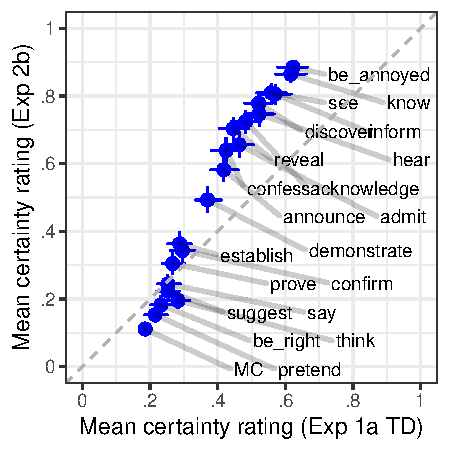
\includegraphics[width=\textwidth]{../../results/projection-comparisons/graphs/projection-comparison-35}
\caption{Exp.~2b vs.\ Exp.~1a TD.}
\label{f-projcomp1}
\end{subfigure}
\begin{subfigure}{.33\textwidth}
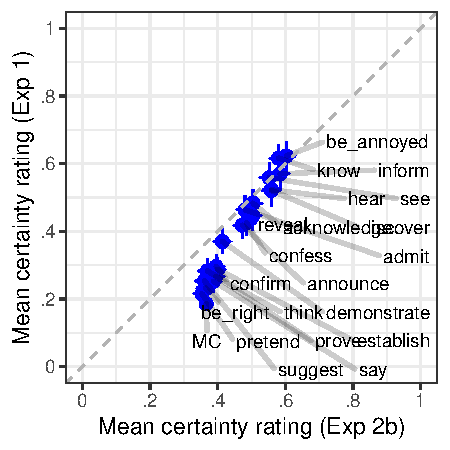
\includegraphics[width=\textwidth]{../../results/projection-comparisons/graphs/projection-comparison-39}
\caption{Exp.~1 vs.\ Exp.~2b.}
\label{f-projcomp2}
\end{subfigure}
\begin{subfigure}{.33\textwidth}
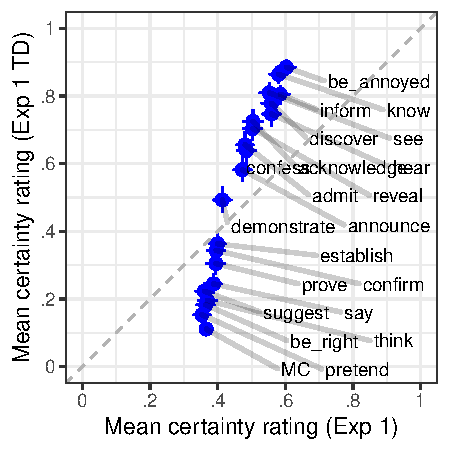
\includegraphics[width=\textwidth]{../../results/projection-comparisons/graphs/projection-comparison-59}
\caption{Exp.~1a TD vs.\  Exp.~1.}
\label{f-projcomp3}
\end{subfigure}
\caption{Comparisons of mean by-predicate certainty ratings from Exp.~1, Exp.~2b, and Tonhauser \& Degen's Exp.~1a (abbreviated `Exp.~1a TD'). Error bars indicate 95\% bootstrapped confidence intervals.}
\label{f-projection-comparisons}
\end{figure}

\section{Prior probability results in Exp.~2a}\label{a-exp2}

\figref{f-prior-2a} plots the mean prior probabilities of the 20 contents by fact. Participants' ratings are given as light dots. The mean prior probability rating for each content was higher when the content was presented with the higher probability fact than when it was presented with the lower probability fact.

\begin{figure}[h!]
\centering
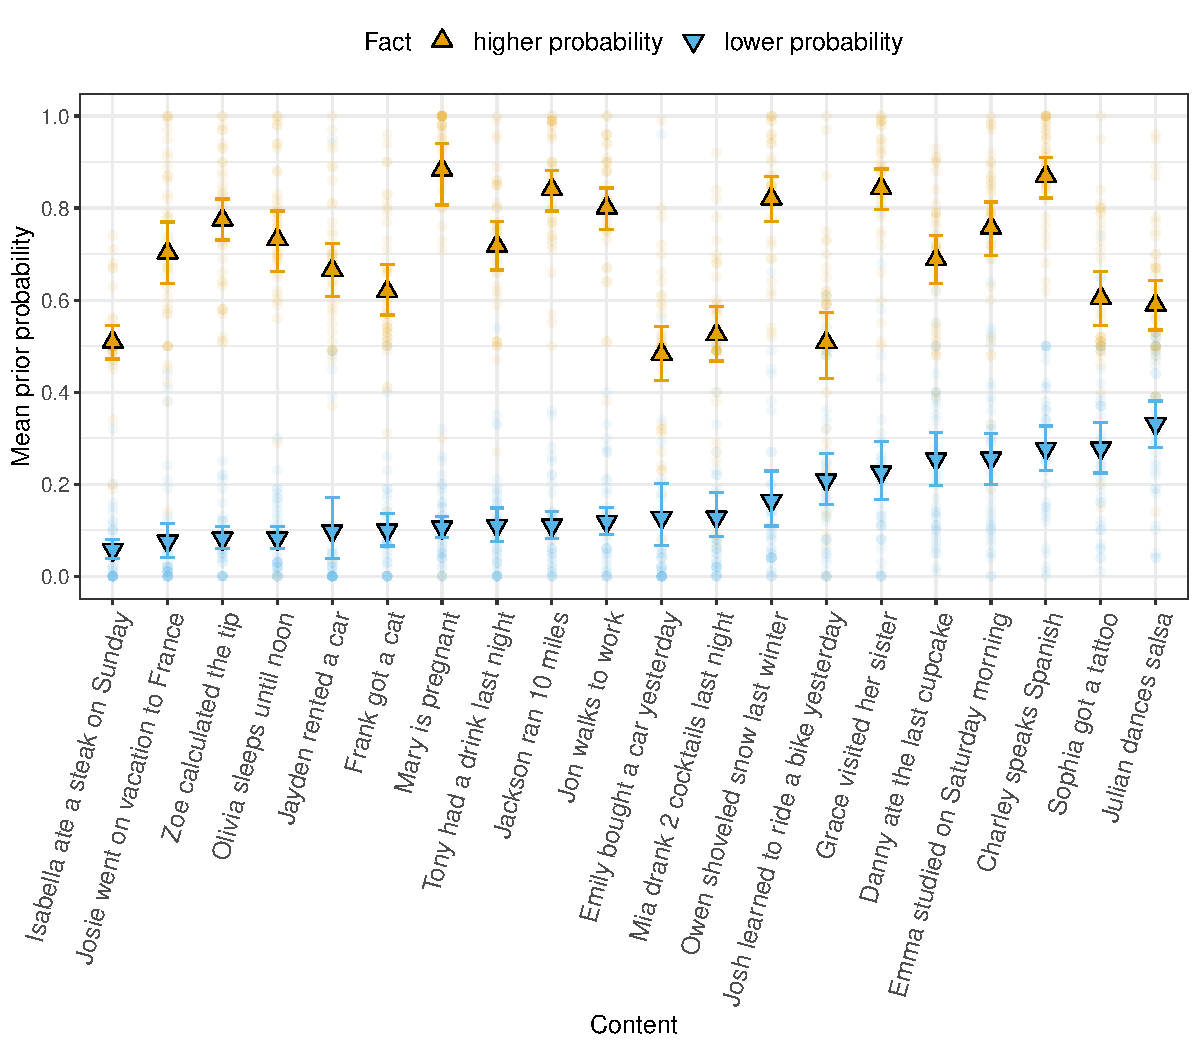
\includegraphics[width=.75\paperwidth]{../../results/1-prior/graphs/prior-ratings}

\caption{Mean prior probability by content and fact in Exp.~2a. Error bars indicate 95\% bootstrapped confidence intervals. Light dots indicate participants' ratings.} 
\label{f-prior-2a}
\end{figure}


\end{document}

